\documentclass[12pt]{article}

% UTF-8 encoding and fonts
\usepackage[utf8]{inputenc}
\usepackage[T1]{fontenc}
\usepackage{lmodern}  % Latin Modern font - fixes < > rendering issues

% Page setup
\usepackage[margin=1in]{geometry}
\usepackage{setspace}
\onehalfspacing

% Typography
\usepackage{microtype}

% Math and symbols
\usepackage{amsmath,amssymb}

% Graphics
\usepackage{graphicx}
\usepackage{float}
\usepackage{subcaption}

% Tables
\usepackage{booktabs}
\usepackage{array}
\usepackage{multirow}
\usepackage{threeparttable} % provides tablenotes
\usepackage{longtable}
\usepackage{pdflscape}
\usepackage{siunitx}
\sisetup{detect-all=true, group-separator={,}, group-minimum-digits=4}

% Bibliography
\usepackage{natbib}
\bibliographystyle{aer}  % American Economic Review style

% Hyperlinks
\usepackage{hyperref}
\hypersetup{
    colorlinks=true,
    linkcolor=blue,
    citecolor=blue,
    urlcolor=blue
}
\usepackage[nameinlink,noabbrev]{cleveref}

% Timing data (generated by timing_log.py)
\IfFileExists{timing_data.tex}{\input{timing_data.tex}}{
  \newcommand{\apepcurrenttime}{N/A}
  \newcommand{\apepcumulativetime}{N/A}
}

% Captions
\usepackage{caption}
\captionsetup{font=small,labelfont=bf}

% Section formatting
\usepackage{titlesec}
\titleformat{\section}{\large\bfseries}{\thesection.}{0.5em}{}
\titleformat{\subsection}{\normalsize\bfseries}{\thesubsection}{0.5em}{}

% Custom commands
\newcommand{\E}{\mathbb{E}}
\newcommand{\Var}{\text{Var}}
\newcommand{\Cov}{\text{Cov}}
\newcommand{\ind}{\mathbb{I}}
\newcommand{\sym}[1]{\ifmmode^{#1}\else\(^{#1}\)\fi}

\title{Cash Scarcity and Food Markets: Evidence from Nigeria's 2023 Currency Redesign}
\author{APEP Autonomous Research\thanks{Autonomous Policy Evaluation Project. Correspondence: scl@econ.uzh.ch{} (cumulative: \apepcumulativetime{}).} \and @olafdrw}
\date{\today}

\begin{document}

\maketitle

\begin{abstract}
\noindent
How does a sudden cash scarcity affect food markets in a developing economy? We study Nigeria's 2023 currency redesign, in which the Central Bank withdrew existing banknotes with only months' notice, creating severe cash shortages. Using cross-state variation in banking infrastructure density as a proxy for differential exposure, we estimate a continuous difference-in-differences model on weekly food prices from 13 Nigerian states over 2019--mid-2024. We find no robust relationship between banking-density-based exposure and food price changes during the crisis ($\beta = -0.16$, $p = 0.21$; wild cluster bootstrap $p = 0.52$). This null holds with state-specific linear trends, a North-South dummy, and randomization inference. Placebo tests reveal pre-existing differential trends along the banking gradient, limiting causal interpretation. We document these identification challenges as a cautionary case for continuous DiD designs where treatment intensity proxies correlate with deep structural differences across units.
\end{abstract}

\vspace{1em}
\noindent\textbf{JEL Codes:} E42, O12, Q11, D04 \\
\noindent\textbf{Keywords:} currency redesign, demonetization, food prices, cash scarcity, Nigeria

\newpage

\section{Introduction}

In early 2023, the price of a 1,000-naira note in parts of Nigeria was 1,200 naira. This 20\% premium---the literal cost of holding cash---was the visible symptom of a currency redesign that had drained the economy of its medium of exchange. On October 26, 2022, the Central Bank of Nigeria (CBN) announced that all existing 200, 500, and 1,000 naira banknotes would cease to be legal tender by January 31, 2023. Citizens had roughly three months to deposit old notes and obtain newly designed currency. ATMs ran dry, bank queues stretched for blocks, and millions of Nigerians who depended on physical cash for daily transactions found themselves unable to buy food, fuel, or basic necessities. Protests erupted in multiple cities. The Supreme Court eventually intervened, extending the deadline, but the damage was done: for several weeks in early 2023, large parts of the Nigerian economy operated under severe cash scarcity.

This paper asks a simple question: did the naira redesign crisis \textit{differentially} affect food prices across Nigerian states as a function of local banking infrastructure? We emphasize ``differentially'': our design, which includes week fixed effects, absorbs any aggregate effect of the crisis common to all states. We can only detect effects that vary with banking density---not the overall impact of the redesign on food prices. The answer matters for both monetary policy and food security. Nigeria is Africa's most populous country, with over 200 million people. The majority of retail food transactions occur in cash. If a sudden withdrawal of physical currency disrupts food markets more severely in areas with fewer banks and ATMs, then the distributional consequences of monetary interventions are mediated by financial infrastructure in ways that standard macroeconomic models do not capture.

We bring this question to the data using a continuous difference-in-differences (DiD) design inspired by \citet{chodorow2020cash}, who studied India's 2016 demonetization by exploiting cross-district variation in pre-demonetization currency holdings. Our setting is analogous but distinct. We measure treatment intensity as a continuous index of ``cash scarcity''---the standardized inverse of bank branches per 100,000 population in each state. States with fewer branches per capita had lower capacity to distribute new banknotes and process old-note deposits, and thus experienced more severe cash shortages. We interact this cross-sectional intensity measure with an indicator for the acute crisis period (February 1 through March 6, 2023) and estimate the effect on a state-level food price index constructed from weekly FEWS NET commodity price data across 13 Nigerian states.

Our main finding is a null result. The point estimate on the interaction of cash scarcity with the crisis indicator is $-0.16$ log points, suggesting that more cash-scarce states experienced slightly \textit{lower} food prices during the crisis---the opposite of what standard models would predict. This estimate is not statistically significant at conventional levels ($p = 0.21$ with cluster-robust standard errors). The null is robust to alternative inference procedures: a wild cluster bootstrap following \citet{webb2022reworking} yields $p = 0.52$, and randomization inference in the spirit of \citet{fisher1935design} produces $p = 0.24$. The result holds across alternative treatment windows, conflict controls, and separate announcement and crisis period indicators.

We probe this null in several dimensions. A commodity-level analysis reveals that food prices---whether grains, legumes and tubers, or processed foods like bread---show no significant differential response to banking density during the crisis. Fuel prices, however, tell a different story: states with greater cash scarcity experienced significantly \textit{higher} fuel price increases ($\beta = 0.17$, $p = 0.02$). This asymmetry is consistent with the hypothesis that fuel markets, which are more formalized and involve larger per-transaction values, were differentially affected by banking access, while food markets---dominated by small-scale, informal, open-air trading---adapted through alternative exchange mechanisms. A dose-response analysis using quintiles of banking density reveals a non-monotonic pattern that further undermines the continuous treatment assumption.

We are transparent about the limitations of our identification strategy. Placebo tests reveal that several pre-crisis dates also produce significant coefficients when used as pseudo-treatment dates, suggesting pre-existing differential trends between high- and low-banking-density states. This is a fundamental threat to the continuous DiD design: if food price dynamics systematically differed across states along the banking density gradient \textit{before} the naira crisis, then the parallel trends assumption is violated, and the main estimate cannot be interpreted causally. We discuss what this means for inference and argue that the placebo failures, combined with the null main result, suggest that the banking density gradient does not provide clean identification of the cash scarcity channel in this setting.

This paper contributes to several literatures. First, we contribute to the emerging literature on the real effects of demonetization and currency withdrawal. The closest comparison is \citet{chodorow2020cash}, who found that Indian districts more exposed to demonetization experienced significantly larger declines in economic activity, credit, and nightlights. Our null finding for Nigeria's food prices does not contradict theirs but highlights an important difference: India's demonetization affected 86\% of currency in circulation overnight, while Nigeria's redesign was phased and affected a smaller share of notes. Moreover, the \citet{chodorow2020cash} framework exploits granular \textit{district-level} variation in pre-demonetization cash holdings from the Reserve Bank of India, while our banking density measure is a noisier state-level proxy that may not capture the relevant margin of cash scarcity.

Second, we contribute to the literature on food price determination in developing countries \citep{deaton1989rice, atkin2015trade, aker2010information, jensen2007digital}. A large body of work has examined how information, transportation costs, and market integration affect food price levels and dispersion. We add to this literature by examining a different channel: the destruction of the medium of exchange itself. Our null result on food prices, combined with the significant fuel price effect, suggests that informal food markets in West Africa possess considerable resilience to monetary disruptions, perhaps because of the pervasiveness of informal credit, barter, and community-level risk-sharing mechanisms that substitute for cash in times of scarcity.

Third, we contribute to the literature on financial inclusion and monetary transmission in developing economies \citep{jack2014risk, suri2017long, aker2017payment}. The finding that banking infrastructure density does not predict differential food price responses to the cash crisis raises questions about the extent to which formal financial access mediates the real effects of monetary policy in contexts where informal institutions are strong. This echoes \citet{jack2014risk}, who documented the role of mobile money in smoothing consumption shocks in Kenya, and suggests that the relationship between formal finance and real economic resilience is complex and context-dependent.

Fourth, from a methodological perspective, we contribute a cautionary case for continuous DiD designs in settings where the treatment intensity proxy correlates with deep structural differences across units. The banking density gradient in Nigeria maps almost perfectly onto the North-South divide, generating pre-existing differential trends that confound identification. Our placebo test failures are not incidental---they reveal a fundamental challenge for difference-in-differences designs that exploit geographic variation in financial infrastructure as a proxy for monetary policy exposure. We document this challenge transparently, including the multiple reasons why the null may obtain---aggregate channels, measurement error, and violated parallel trends---and argue that each explanation is itself informative.

The remainder of the paper is organized as follows. Section 2 describes the institutional background of the naira redesign, including the timeline of events, the severity of the cash crisis, and the structure of Nigeria's banking sector. Section 3 develops a simple conceptual framework that generates predictions about the effect of cash scarcity on food prices. Section 4 describes our data sources and variable construction. Section 5 presents the empirical strategy. Section 6 reports the main results, including event studies, commodity heterogeneity, and dose-response analysis. Section 7 presents robustness checks and discusses threats to identification. Section 8 offers a discussion of why the null result obtains and what it implies for policy. Section 9 concludes.


\section{Institutional Background}

\subsection{The Naira Redesign Policy}

Nigeria's currency redesign was announced by CBN Governor Godwin Emefiele on October 26, 2022 \citep{cbn2022redesign}. The stated objectives were threefold: to curb counterfeiting and hoarding of large-denomination notes, to encourage the transition to a cashless economy, and to rein in election-related illicit cash flows ahead of the February 2023 general elections. The CBN ordered that all existing 200, 500, and 1,000 naira notes be returned to banks by January 31, 2023, after which they would cease to be legal tender. Newly redesigned notes with updated security features would replace them.

The policy was ambitious in scope. The three affected denominations accounted for over 80\% of the value of currency in circulation, estimated at approximately 3.2 trillion naira (roughly \$7 billion) at the time of the announcement. The CBN initially imposed a weekly withdrawal limit of 500,000 naira for individuals and 5 million naira for businesses, which was subsequently reduced to 100,000 naira and 500,000 naira respectively as the deadline approached. These limits, combined with insufficient printing and distribution of new notes, created the conditions for a severe cash squeeze.

The timeline of the crisis can be divided into three phases. The \textit{announcement phase} (October 26, 2022 to January 30, 2023) saw a gradual increase in cash deposits as Nigerians rushed to return old notes. Banks struggled to process the volume, with long queues becoming commonplace. The \textit{acute crisis phase} (January 31 to approximately March 6, 2023) was characterized by extreme cash scarcity. Many ATMs were non-functional or empty. Point-of-sale (POS) terminals charged premiums of 10--20\% for cash withdrawals. The mobile money platform and bank transfer system experienced frequent outages due to unprecedented demand. Protests erupted in Abuja, Lagos, Ibadan, and Benin City. On February 8, 2023, President Buhari extended the deadline to February 10 for the old 200 naira note only. The Supreme Court intervened on March 3, ruling that the old notes must remain legal tender until December 31, 2023. The \textit{resolution phase} (March 7 onward) saw a gradual return to normalcy as old notes re-entered circulation and new notes became more widely available.

The crisis disproportionately affected rural areas and states with limited banking infrastructure. Nigeria's banking sector is heavily concentrated in the commercial hubs of Lagos, Abuja, and the southern states. Northern states, which are predominantly agrarian and have vastly fewer bank branches per capita, faced the most severe shortages. In Zamfara state, for example, there were only 0.5 bank branches per 100,000 people, compared to 8.1 per 100,000 in Lagos---a sixteen-fold difference. This cross-state variation in banking density provides the basis for our identification strategy.

\subsection{Nigeria's Banking Infrastructure}

Nigeria's formal financial sector is characterized by extreme geographic concentration. As of 2022, the country had approximately 5,700 branches of deposit money banks (DMBs), serving a population of over 200 million \citep{cbn2023banking}. The distribution of these branches is highly uneven. Lagos state alone accounts for approximately 22\% of all bank branches nationwide, despite containing only 7\% of the population. The six states of the geopolitical South-West zone contain more bank branches than the entire 19-state North.

This geographic imbalance in financial infrastructure has deep historical roots. Colonial-era banking was concentrated in the ports of Lagos and Calabar. Post-independence financial liberalization in the 1990s led to rapid branch expansion, but overwhelmingly in commercially viable urban centers. The 2005 banking consolidation, which raised the minimum capital requirement from 2 billion to 25 billion naira, eliminated many smaller banks that had served rural communities. By 2022, Nigeria's banking sector was dominated by 22 commercial banks, the largest of which operated primarily in the Southwest and Northcentral zones.

Mobile money and alternative financial services have expanded rapidly since the CBN licensed mobile money operators in 2021, but penetration remains low in rural northern states. According to the World Bank's Global Findex database, as of 2021, only 40\% of Nigerian adults had a bank account, and only 6\% had used mobile money in the past year \citep{wbdi2024}. The cash economy thus remained dominant for most Nigerians at the time of the redesign. Open-air markets, where the bulk of food retail occurs, were almost exclusively cash-based. Traders in these markets typically lacked POS terminals and had limited access to digital payment infrastructure.

\subsection{Food Markets and Pricing in Nigeria}

Nigeria's food markets are overwhelmingly informal. The retail food sector is dominated by open-air markets, roadside stalls, and itinerant traders. Supply chains for staple foods---maize, millet, sorghum, rice, cowpeas, yams, cassava, and gari (processed cassava)---are long and fragmented, typically involving multiple intermediaries between the farm gate and the final consumer. Transportation costs are a major component of food prices, as Nigeria's road infrastructure is poor and fuel costs are high \citep{atkin2015trade}.

Food prices in Nigeria exhibit substantial spatial dispersion. Prices for the same commodity can differ by a factor of two or more across states, reflecting transportation costs, local supply conditions, and market power of intermediaries. Prices are also highly seasonal, with harvest periods bringing temporary price declines that are gradually eroded by storage costs and supply depletion. The naira redesign occurred during the dry season, a period of typically rising food prices as stored grains and tubers are drawn down and the new planting season has not yet begun.

The FEWS NET (Famine Early Warning Systems Network) has collected weekly commodity prices in Nigerian markets since 2017. The FEWS NET price monitoring system covers approximately 40 markets across 15 states, tracking prices for 20 staple food commodities and fuel. These data, described in detail in Section 4, form the backbone of our empirical analysis.


\section{Conceptual Framework}

We develop a simple framework to structure our empirical analysis. Consider a stylized model of a local food market in state $s$ at time $t$. The equilibrium price $P_{st}$ is determined by the intersection of supply and demand:
\begin{equation}
    P_{st} = f(D_{st}, S_{st}, M_{st})
\end{equation}
where $D_{st}$ denotes demand conditions, $S_{st}$ denotes supply conditions, and $M_{st}$ captures the state of the monetary/payment system. In a cash-dependent economy, $M_{st}$ reflects the availability of physical currency as a medium of exchange.

A sudden reduction in cash availability---such as that caused by the naira redesign---can affect food prices through several channels. We distinguish between \textit{demand-side} and \textit{supply-side} channels, and between \textit{aggregate} and \textit{differential} effects.

\textbf{Demand-side channel.} Cash scarcity reduces consumers' ability to purchase food. If consumers cannot access cash and lack alternative payment mechanisms, effective demand falls, putting downward pressure on food prices. This channel predicts $\partial P / \partial M > 0$ (less cash $\Rightarrow$ lower demand $\Rightarrow$ lower prices), and should operate more strongly in states with lower banking density where alternative payment mechanisms are less available.

\textbf{Supply-side channel.} Cash scarcity also affects sellers and intermediaries. If traders cannot pay farmers, transporters, or wholesalers in cash, supply chains may be disrupted, reducing the quantity of food reaching retail markets. This channel predicts $\partial P / \partial M < 0$ (less cash $\Rightarrow$ lower supply $\Rightarrow$ higher prices), and should also vary with banking infrastructure.

\textbf{Aggregate versus differential effects.} Critically, the naira redesign was a nationwide policy shock. All states were affected simultaneously. If the crisis operates primarily through aggregate channels---nationwide supply chain disruption, general macroeconomic uncertainty, changes in central bank policy---then food prices should move together across states regardless of banking density. In this case, state and week fixed effects absorb the effect, and the interaction of banking density with the crisis indicator is zero. Only if the crisis operates through \textit{differential} channels---with banking density mediating the local severity of the shock---should we observe a non-zero interaction coefficient.

This generates our testable predictions:

\textit{Prediction 1: Differential effect.} If cash scarcity affects food prices differentially across states, the interaction of the cash scarcity index with the crisis indicator should be non-zero. The sign depends on whether demand-side or supply-side channels dominate.

\textit{Prediction 2: Commodity heterogeneity.} The differential effect should be stronger for commodities traded in more formalized markets (where cash constraints bind more tightly) and weaker for commodities traded in highly informal settings (where barter and informal credit can substitute for cash).

\textit{Prediction 3: Aggregate null.} If the crisis operates primarily through aggregate channels, the interaction coefficient should be approximately zero, and the effect of the crisis should be absorbed by time fixed effects.

Our main results are most consistent with Prediction 3, though we cannot rule out that measurement error in the treatment variable or violations of parallel trends also contribute to the null.


\section{Data}

To measure how these cash-starved markets responded, we assemble three data sources: weekly food price data collected by trained monitors in open-air markets (FEWS NET), bank branch counts from the Central Bank of Nigeria, and conflict event data from the Uppsala Conflict Data Program (UCDP).

\subsection{FEWS NET Food Prices}

Our primary outcome data come from the Famine Early Warning Systems Network (FEWS NET), which collects weekly commodity prices from markets across Nigeria \citep{fewsnet2024}. The FEWS NET price monitoring system tracks prices for approximately 20 staple food commodities and fuel across 15 Nigerian states. The commodities include major grains (maize, millet, sorghum, rice), legumes (cowpeas), tubers (yams, cassava, gari), processed foods (bread), and fuel (diesel, petrol). Prices are reported in Nigerian naira per kilogram (or per liter for fuel) and represent retail market prices collected by trained monitors.

We access the FEWS NET data through their public API, obtaining 305,288 individual price observations covering the period from January 2019 through mid-2024. We restrict our analysis to states with consistent price reporting over this period, yielding an unbalanced panel of 13 states spanning 279 weeks (January 2019 through May 2024), with $N = 3{,}492$ state-week observations. The panel is unbalanced because some states have occasional gaps in weekly reporting; Abia state, for example, has 167 observed weeks out of 279 due to intermittent monitoring. The raw data include price observations for multiple commodities and multiple markets within each state-week cell.

To construct our primary dependent variable, we aggregate the raw commodity prices into a state-level food price index. For each state-week, we compute the geometric mean of available food commodity prices (excluding fuel), yielding a composite index that captures the average level of food prices. We then take the natural logarithm of this index. The resulting variable, $\ln(\text{FoodPriceIndex}_{st})$, is our primary outcome.

\subsection{Banking Infrastructure Data}

Our treatment intensity measure is constructed from the Central Bank of Nigeria's list of deposit money bank (DMB) branches by state \citep{cbn2023banking}. For each of the 13 FEWS NET states in our sample, we record the number of DMB branches and compute the ratio of branches to population (per 100,000). We then construct a continuous ``cash scarcity'' index defined as:
\begin{equation}
    \text{CashScarcity}_s = 1 - \frac{\text{Branches/100k}_s - \min(\text{Branches/100k})}{\max(\text{Branches/100k}) - \min(\text{Branches/100k})}
\end{equation}
This index ranges from 0 (highest banking density, i.e., Lagos) to 1 (lowest banking density, i.e., Zamfara). The cross-state variation is substantial: banking density ranges from 0.5 branches per 100,000 in Zamfara to 8.1 in Lagos, with a mean of 1.66 and a standard deviation of 2.07 (\Cref{tab:summary}).

The cash scarcity index is time-invariant and measured prior to the crisis. This is essential for identification: we exploit pre-existing cross-sectional variation in banking infrastructure, not endogenous changes in banking access during the crisis. The assumption is that states with fewer bank branches per capita had lower capacity to distribute new currency and thus experienced more severe cash shortages during the redesign---a reasonable assumption given the logistical constraints of new-note distribution.

\subsection{Conflict Data}

We control for local conflict intensity using event-level data from the Uppsala Conflict Data Program (UCDP) \citep{sundararaman2023ucdp}. Northern Nigeria has experienced significant armed conflict, including the Boko Haram insurgency in the Northeast and banditry in the Northwest. These security conditions may independently affect food prices through supply chain disruptions and market closures. We geo-locate UCDP conflict events to Nigerian states and construct a monthly count of conflict events per state. The UCDP GED v24.1 covers events through December 2023; for the January--May 2024 portion of our sample, conflict counts are set to zero. Since our identification exploits variation around February 2023, the 2024 coding does not affect any key estimate. Over the 2019--2023 portion of our sample, we observe 9,787 conflict events across Nigeria, with a mean of 2.3 events per state-month and substantial cross-state variation.

\subsection{Summary Statistics}

\Cref{tab:summary} reports summary statistics for our key variables. Panel A describes state-level characteristics. The 13 states in our sample have a mean population of 7.1 million and an average of 163 bank branches. Banking density varies enormously, from 0.5 to 8.1 branches per 100,000, with a mean of 1.66. The cash scarcity index averages 0.91, reflecting the fact that most states in the FEWS NET sample are in the banking-sparse North.

Panel B describes the food price and control variables. The mean log food price index was 7.77 in the pre-crisis period (before February 2023), rose to 8.08 during the acute crisis, and increased further to 8.36 in the post-crisis period. This substantial increase reflects the combination of the cash crisis, general inflation, and the typical seasonal pattern of rising food prices during the dry season. The average state-week observation includes prices for 16.4 of the 20 tracked commodities. Conflict intensity averages 2.3 events per state-month.

\begin{table}[H]
\centering
\caption{Summary Statistics}
\begin{threeparttable}
\begin{tabular}{lS[table-format=3.2]S[table-format=3.2]S[table-format=2.2]S[table-format=4.0]}
\toprule
Variable & {Mean} & {Std.\ Dev.} & {Min} & {Max} \\
\midrule
\multicolumn{5}{l}{\textit{Panel A: State Characteristics ($N = 13$ states)}} \\
\addlinespace
Bank branches (count)          & 163.23 & 329.76 & 23.00 & 1247 \\
Population (millions)          & 7.10   & 3.72   & 3.42  & {15.39} \\
Branches per 100k pop.         & 1.66   & 2.07   & 0.51  & {8.10} \\
Cash scarcity index (0--1)     & 0.91   & 0.16   & 0.41  & {1.00} \\
\addlinespace
\multicolumn{5}{l}{\textit{Panel B: Food Prices and Controls ($N = 3{,}492$ state-weeks)}} \\
\addlinespace
Log food price index (pre-crisis)  & 7.77  & 0.42  & 4.61  & {9.54} \\
Log food price index (crisis)      & 8.08  & 0.19  & 7.63  & {8.47} \\
Log food price index (post-crisis) & 8.36  & 0.23  & 5.70  & {8.86} \\
Products per state-week            & 16.40 & 2.16  & 1.00  & {20} \\
Conflict events (state-month)      & 2.35  & 7.39  & 0.00  & {61} \\
\bottomrule
\end{tabular}
\begin{tablenotes}[flushleft]
\small
\item \textit{Notes:} Panel A reports cross-sectional state characteristics. Panel B reports state-week level observations. The food price index is the geometric mean of available commodity prices (excluding fuel) in each state-week. Cash scarcity is the min-max normalized inverse of bank branches per 100,000 population. Crisis = Feb 1 -- Mar 6, 2023.
\end{tablenotes}
\end{threeparttable}
\label{tab:summary}
\end{table}


\section{Empirical Strategy}

\subsection{Identification}

Our identification strategy follows the continuous difference-in-differences framework of \citet{chodorow2020cash}. The key insight is that the naira redesign was a nationwide policy shock, but its severity varied across states as a function of pre-existing banking infrastructure. States with fewer bank branches per capita had lower capacity to distribute new currency and thus experienced more severe cash shortages. We exploit this cross-state variation in treatment intensity to estimate the differential effect of cash scarcity on food prices.

Our baseline estimating equation is:
\begin{equation}
\ln(\text{FoodPrice}_{st}) = \alpha_s + \gamma_t + \beta \cdot \text{CashScarcity}_s \times \text{Crisis}_t + \varepsilon_{st}
\label{eq:main}
\end{equation}
where $\ln(\text{FoodPrice}_{st})$ is the log food price index in state $s$ and week $t$; $\alpha_s$ are state fixed effects, which absorb all time-invariant differences across states (including baseline levels of banking density, income, urbanization, and agricultural productivity); $\gamma_t$ are week fixed effects, which absorb all aggregate shocks common to all states in a given week (including nationwide inflation, exchange rate movements, and the aggregate effect of the naira crisis itself); $\text{CashScarcity}_s$ is the continuous treatment intensity measure described in Section 4.2; and $\text{Crisis}_t$ is an indicator equal to one during the acute crisis period (February 1 through March 6, 2023).

The coefficient of interest is $\beta$, which captures the differential change in food prices during the crisis associated with a one-unit increase in cash scarcity. Under the null hypothesis that the crisis affected all states equally regardless of banking density, $\beta = 0$. Under the alternative that banking infrastructure mediated the local severity of the cash crisis, $\beta \neq 0$.

We estimate Equation \ref{eq:main} using OLS with standard errors clustered at the state level to account for serial correlation within states \citep{bertrand2004much}. With only 13 clusters, standard cluster-robust inference may be unreliable \citep{cameron2008bootstrap}. We therefore supplement our main results with two alternative inference procedures: the wild cluster bootstrap with Webb's six-point distribution \citep{webb2022reworking, mackinnon2018wild} and randomization inference \citep{fisher1935design}.

\subsection{Alternative Specifications}

We estimate several variants of Equation \ref{eq:main} to probe the robustness of our findings. First, we replace the acute crisis indicator with a broader post-deadline indicator (all weeks after January 30, 2023) to capture persistent effects. Second, we add controls for local conflict intensity ($\ln(1 + \text{ConflictEvents}_{st})$) to address the concern that security conditions may confound the relationship between banking density and food prices. Third, we separately interact cash scarcity with indicators for the announcement phase (October 26, 2022 to January 30, 2023) and the acute crisis phase to test for anticipation effects.

We also conduct several diagnostic exercises. An event-study specification replaces the single crisis indicator with a full set of week-by-cash-scarcity interactions, allowing us to visualize the time path of the differential effect and assess the plausibility of the parallel trends assumption. A commodity-level analysis estimates Equation \ref{eq:main} separately for major commodity groups (grains, legumes and tubers, processed foods, and fuel) to examine heterogeneity in the price response. A dose-response analysis replaces the continuous cash scarcity measure with indicators for quintiles of banking density to test for non-linearity.

\subsection{Identification Assumptions and Threats}

The causal interpretation of $\beta$ requires two key assumptions. First, \textit{parallel trends}: in the absence of the naira crisis, food prices in high- and low-banking-density states would have evolved along parallel trajectories. Second, \textit{no differential confounders}: no other shock correlated with both banking density and food prices occurred simultaneously with the crisis.

We assess the parallel trends assumption in three ways. The event-study specification allows visual inspection of pre-treatment differential trends. Placebo tests estimate Equation \ref{eq:main} with pseudo-treatment dates in the pre-crisis period. And we discuss whether the \citet{rambachan2023more} sensitivity analysis framework applies to our continuous-treatment setting.

Several threats to identification merit discussion. First, banking density is correlated with urbanization, income, and economic development. While state fixed effects absorb time-invariant differences in these variables, they do not absorb differential time trends. If wealthier, more urbanized states experienced different food price trajectories for reasons unrelated to the cash crisis, the parallel trends assumption is violated. Our placebo tests are designed to detect exactly this threat.

Second, the naira redesign coincided with the February 2023 general elections, which may have independently affected food markets through campaign spending, security operations, or economic uncertainty. To the extent that election effects were common across states, they are absorbed by week fixed effects. But if election-related disruptions varied systematically with banking density, our estimate is confounded.

Third, our treatment intensity measure---banking density---is a proxy for the true treatment of interest---local cash scarcity. Measurement error in this proxy will attenuate our estimate toward zero, potentially contributing to the null result. We lack direct data on cash availability by state during the crisis, which is a limitation shared with much of the demonetization literature.

Fourth, with only 13 states (clusters), our statistical power is limited. We discuss minimum detectable effects in the context of our results and acknowledge that the null may reflect insufficient power rather than a true zero effect.


\section{Results}

\subsection{Main Results}

Food prices were remarkably unresponsive to the local severity of the cash shortage. \Cref{tab:main} presents our main estimates. In the baseline specification (Column 1), states with the most severe cash scarcity experienced food prices that were, if anything, slightly \textit{lower} during the crisis than states with abundant banking ($\hat{\beta} = -0.160$, SE $= 0.120$, $p = 0.206$)---the opposite of what standard models would predict. The estimate is not statistically significant at any conventional level. The within-$R^2$ of 0.0004 indicates that local banking infrastructure explains essentially none of the residual variation in food prices once aggregate shocks are absorbed by week fixed effects.

Extending the crisis window to the full post-deadline period (Column 2) does not change the picture. The coefficient reverses sign ($\hat{\beta} = 0.091$, SE $= 0.097$, $p = 0.367$), and the sign instability itself is informative: there is no stable differential food price response to local banking density, regardless of how the crisis period is defined.

Adding conflict controls (Column 3) leaves the result unchanged ($\hat{\beta} = -0.151$, SE $= 0.124$, $p = 0.248$). Armed violence---despite its severity in northern Nigeria---does not confound the cash scarcity coefficient in this specification.

Separating the announcement and acute crisis phases (Column 4) reveals no anticipation effects ($\hat{\beta}_{\text{announce}} = 0.086$, $p = 0.35$) and a larger but still insignificant crisis coefficient ($\hat{\beta}_{\text{crisis}} = -0.222$, $p = 0.16$). The reversal in sign between phases undermines any coherent narrative of gradual build-up followed by acute disruption.

\begin{table}[H]
\centering
\caption{The Effect of Cash Scarcity on Food Prices}
\begin{threeparttable}
\begin{tabular}{lcccc}
\toprule
& (1) & (2) & (3) & (4) \\
& Acute Crisis & Post-Deadline & Conflict Control & Two-Phase \\
\midrule
Cash Scarcity $\times$ Crisis & $-0.160$ & & $-0.151$ & $-0.222$ \\
& $(0.120)$ & & $(0.124)$ & $(0.149)$ \\
Cash Scarcity $\times$ Post-Deadline & & $0.091$ & & \\
& & $(0.097)$ & & \\
Log(1 + Conflict Events) & & & $0.011$ & \\
& & & $(0.015)$ & \\
Cash Scarcity $\times$ Post-Announce & & & & $0.086$ \\
& & & & $(0.088)$ \\
\addlinespace
State FE & Yes & Yes & Yes & Yes \\
Week FE & Yes & Yes & Yes & Yes \\
\addlinespace
Observations & 3,492 & 3,492 & 3,492 & 3,492 \\
Within $R^2$ & 0.0004 & 0.0014 & 0.0013 & 0.0017 \\
$R^2$ & 0.891 & 0.891 & 0.891 & 0.891 \\
\bottomrule
\end{tabular}
\begin{tablenotes}[flushleft]
\small
\item \textit{Notes:} Standard errors clustered at the state level in parentheses. * $p<0.10$, ** $p<0.05$, *** $p<0.01$. The dependent variable is the log of the state-level food price index. Cash Scarcity is the standardized inverse of bank branches per 100,000 population. Crisis = Feb 1 -- Mar 6, 2023. Post-Deadline = all weeks after Jan 30, 2023. Post-Announce = all weeks after Oct 26, 2022. All specifications include state and week fixed effects. $N = 3{,}492$ state-week observations across 13 states spanning 279 weeks (unbalanced panel).
\end{tablenotes}
\end{threeparttable}
\label{tab:main}
\end{table}

Taken together, the main results in \Cref{tab:main} paint a clear picture: there is no statistically significant differential effect of cash scarcity on food prices during the naira crisis. The point estimates are small relative to their standard errors, the signs are inconsistent across specifications, and the within-$R^2$ values are negligible. We interpret this as evidence that the naira crisis did not differentially affect food prices along the banking density gradient---either because the crisis operated through aggregate channels, because our banking density measure is too noisy to detect the relevant variation, or because the parallel trends assumption does not hold in this setting.

\subsection{Event Study}

\Cref{fig:event_study} presents the event-study specification, which plots the coefficients on the interaction of cash scarcity with weekly indicators for 26 weeks before and after the January 31, 2023 deadline. The event-study serves as a visual test of the parallel trends assumption: if pre-treatment coefficients are close to zero and stable, it supports the identifying assumption that food prices in high- and low-banking-density states were trending similarly before the crisis.

The event-study plot reveals several important features. First, the pre-treatment coefficients show some instability, with occasional spikes that deviate from zero. This is consistent with the placebo test failures reported in Section 7 and raises concerns about the parallel trends assumption. Second, the coefficients during and immediately after the crisis period do not show a clear break from the pre-treatment pattern. There is no sharp, discontinuous shift at the time of the deadline, as one would expect if the cash crisis differentially affected food prices in less-banked states. Third, the confidence intervals are wide throughout, reflecting the limited number of clusters and the high degree of within-state variation in food prices.

\begin{figure}[H]
\centering

\includegraphics[width=0.85\textwidth]{figures/fig2_event_study.pdf}
\caption{Event Study: Differential Food Price Response by Cash Scarcity}
\label{fig:event_study}
\begin{minipage}{0.85\textwidth}
\vspace{0.5em}
\small\textit{Notes:} Figure plots coefficients $\hat{\beta}_k$ from a regression of log food prices on state and week fixed effects and the interaction of cash scarcity with weekly indicators for $k = -26, \ldots, +26$ weeks relative to the Jan 31, 2023 deadline. The reference period is $k = -1$. Shaded band shows 95\% confidence intervals based on state-clustered standard errors.
\end{minipage}
\end{figure}

\subsection{Commodity Heterogeneity}

\Cref{tab:commodity} and \Cref{fig:commodity_hetero} report estimates of Equation \ref{eq:main} separately for major commodity groups. This analysis tests Prediction 2 from our conceptual framework: whether the differential effect of cash scarcity varies across commodity types.

The results reveal a striking pattern. For all food commodity groups---grains ($\beta = -0.132$, $p = 0.22$), legumes and tubers ($\beta = -0.203$, $p = 0.18$), and processed foods such as bread ($\beta = -0.101$, $p = 0.49$)---the coefficients are negative and statistically insignificant. The negative signs are consistent across food categories, suggesting a weak tendency for more cash-scarce states to experience slightly lower food prices during the crisis, but the magnitudes are insufficient for statistical significance.

Fuel prices tell a suggestive but fragile story. The cluster-robust coefficient for fuel is positive and significant at the 5\% level ($\beta = 0.166$, SE $= 0.063$, $p = 0.02$), indicating that states with higher cash scarcity experienced differentially \textit{higher} fuel prices during the crisis. However, this result does not survive few-cluster-robust inference: the wild cluster bootstrap yields $p = 0.47$, substantially above conventional significance thresholds. Given 13 clusters and four commodity groups tested, the cluster-robust significance may reflect the well-documented over-rejection of standard inference with few clusters. We therefore treat this finding as exploratory rather than confirmatory. Nevertheless, the direction is suggestive: fuel markets are more formalized than food markets, with petrol stations requiring larger per-transaction payments and closer links to formal supply chains, making them more plausibly susceptible to banking-density-mediated cash constraints.

\begin{table}[H]
\centering
\caption{Commodity-Level Heterogeneity: Effect of Cash Scarcity During Crisis}
\begin{threeparttable}
\begin{tabular}{lcccc}
\toprule
& Grains & Legumes \& Tubers & Processed & Fuel \\
& (1) & (2) & (3) & (4) \\
\midrule
Cash Scarcity $\times$ Crisis & $-0.132$ & $-0.203$ & $-0.101$ & $0.166$** \\
& $(0.101)$ & $(0.144)$ & $(0.141)$ & $(0.063)$ \\
\addlinespace
State FE & Yes & Yes & Yes & Yes \\
Week FE & Yes & Yes & Yes & Yes \\
Observations & 19,589 & 34,187 & 3,489 & 6,972 \\
\bottomrule
\end{tabular}
\begin{tablenotes}[flushleft]
\small
\item \textit{Notes:} Each column reports a separate regression at the commodity-state-week level. Standard errors clustered at the state level in parentheses. * $p<0.10$, ** $p<0.05$, *** $p<0.01$. Grains include maize, millet, sorghum, and rice. Legumes \& Tubers include cowpeas, yams, cassava, and gari. Processed includes bread. Fuel includes diesel and petrol.
\end{tablenotes}
\end{threeparttable}
\label{tab:commodity}
\end{table}

\begin{figure}[H]
\centering
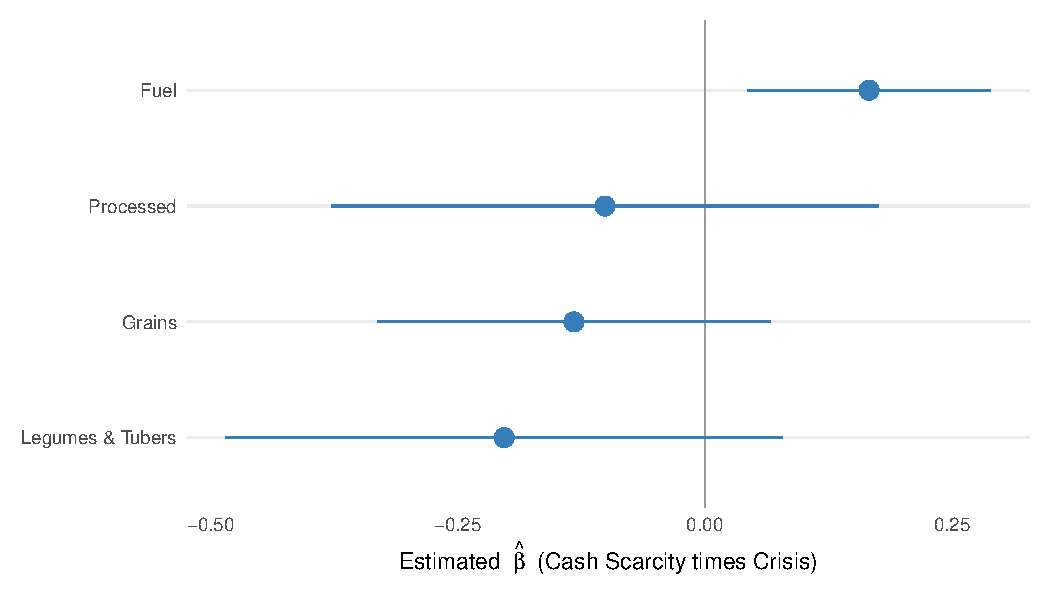
\includegraphics[width=0.75\textwidth]{figures/fig5_commodity_hetero.pdf}
\caption{Commodity-Level Heterogeneity in the Effect of Cash Scarcity}
\label{fig:commodity_hetero}
\begin{minipage}{0.75\textwidth}
\vspace{0.5em}
\small\textit{Notes:} Point estimates and 95\% confidence intervals for the coefficient on Cash Scarcity $\times$ Crisis from separate regressions for each commodity group. The dashed vertical line marks zero.
\end{minipage}
\end{figure}

The food-fuel divergence, while exploratory given the fragility of the fuel result under few-cluster-robust inference, is consistent with the hypothesis that informal food markets possess greater resilience to cash scarcity than more formalized markets. In open-air food markets, traders may extend informal credit to regular customers, accept partial payments, engage in barter, or adjust quantities rather than prices. These informal mechanisms are less available in fuel markets, where transactions are larger, less personal, and more tightly linked to formal supply chains. This interpretation aligns with the broader literature on informal risk-sharing in developing economies \citep{jack2014risk, fafchamps2012soft}, though we emphasize that our evidence is suggestive rather than causal.

\subsection{Dose-Response Analysis}

To test whether the effect of cash scarcity is monotonic---as a continuous treatment model assumes---we estimate a dose-response specification in which we replace the continuous cash scarcity index with indicators for quintiles of banking density. \Cref{fig:dose_response} plots the resulting coefficients relative to the first quintile (lowest banking density).

The dose-response pattern is non-monotonic. Relative to the first quintile (the most cash-scarce states), the second quintile shows a modest negative effect ($\beta_2 = -0.097$, $p = 0.06$), the third quintile is smaller ($\beta_3 = -0.062$, $p = 0.26$), the fourth quintile shows the largest effect ($\beta_4 = -0.200$, $p = 0.004$), and the fifth quintile (least cash-scarce, anchored by Lagos) shows essentially no effect ($\beta_5 = -0.043$, $p = 0.45$).

This non-monotonic pattern is difficult to reconcile with the continuous treatment assumption underlying Equation \ref{eq:main}. If cash scarcity linearly mediated the food price effect of the naira crisis, we would expect a monotonically increasing (or decreasing) pattern across quintiles. Instead, the pattern suggests that banking density captures heterogeneity in state-level food price dynamics that is not well described by a simple linear dose-response relationship. The significant fourth-quintile coefficient may reflect idiosyncratic characteristics of the states in that group rather than a causal effect of intermediate banking density. Lagos, which constitutes the bulk of the fifth quintile and is an extreme outlier in banking density, appears to have evolved similarly to the most cash-scarce northern states---consistent with the aggregate-channel interpretation.

\begin{figure}[H]
\centering
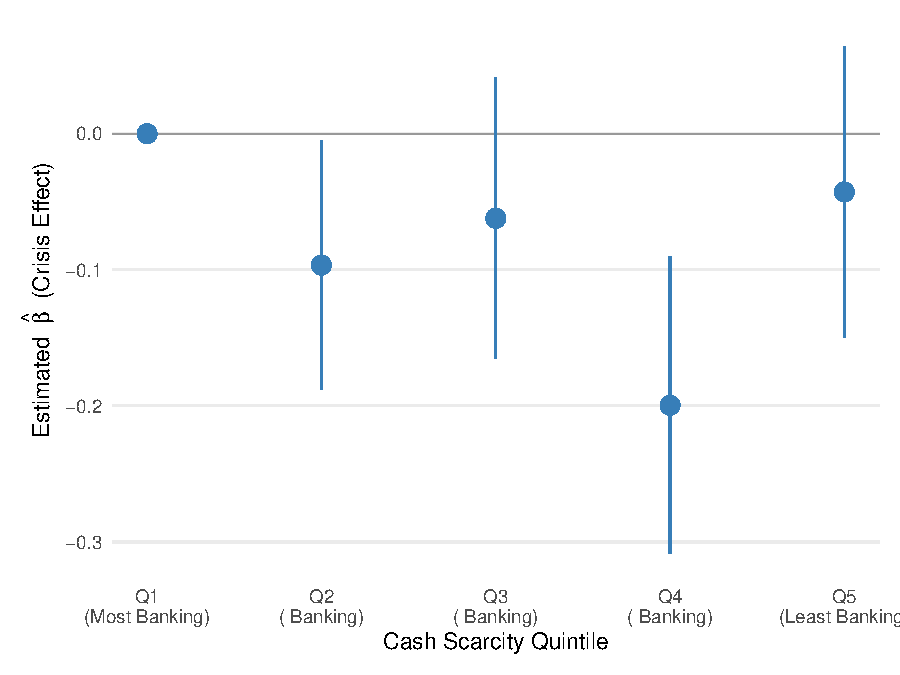
\includegraphics[width=0.75\textwidth]{figures/fig7_dose_response.pdf}
\caption{Dose-Response: Food Price Effects by Banking Density Quintile}
\label{fig:dose_response}
\begin{minipage}{0.75\textwidth}
\vspace{0.5em}
\small\textit{Notes:} Coefficients on quintile indicators interacted with the crisis period, relative to Q1 (lowest banking density). Error bars show 95\% confidence intervals from state-clustered standard errors. The non-monotonic pattern undermines the continuous treatment assumption.
\end{minipage}
\end{figure}


\section{Robustness and Diagnostics}

\subsection{Alternative Inference}

With only 13 clusters, asymptotic cluster-robust standard errors may be unreliable. \Cref{tab:inference} reports our main coefficient under three inference procedures. Cluster-robust standard errors yield $p = 0.206$. The wild cluster bootstrap with Webb's six-point distribution \citep{webb2022reworking, mackinnon2018wild}, which provides better finite-sample performance with few clusters, yields a substantially larger $p$-value of $0.523$. Randomization inference, which permutes the treatment assignment (cash scarcity index) across states and re-estimates Equation \ref{eq:main} for 999 permutations, yields $p = 0.240$.

All three procedures agree: the null cannot be rejected. If anything, the wild cluster bootstrap suggests that the cluster-robust standard errors are too liberal in this setting, consistent with \citet{cameron2008bootstrap}'s finding that cluster-robust inference over-rejects with few clusters. \Cref{fig:ri_distribution} plots the randomization inference distribution alongside the observed test statistic.

\begin{table}[H]
\centering
\caption{Inference Robustness: Main Coefficient Under Alternative Procedures}
\begin{threeparttable}
\begin{tabular}{lcccc}
\toprule
Method & Estimate & $p$-value & 95\% CI & Clusters \\
\midrule
Cluster-Robust SE & $-0.160$ & 0.206 & $[-0.395, 0.075]$ & 13 \\
Wild Cluster Bootstrap (Webb) & $-0.160$ & 0.523 & $[-0.364, 0.047]$ & 13 \\
Randomization Inference & $-0.160$ & 0.240 & --- & 13 \\
\bottomrule
\end{tabular}
\begin{tablenotes}[flushleft]
\small
\item \textit{Notes:} All methods use the baseline specification (Column 1 of \Cref{tab:main}). Wild cluster bootstrap uses 9,999 replications with Webb's six-point weight distribution. Randomization inference uses 999 permutations of the cash scarcity index across states. The WCB confidence interval is the bootstrap percentile interval.
\end{tablenotes}
\end{threeparttable}
\label{tab:inference}
\end{table}

\begin{figure}[H]
\centering

\includegraphics[width=0.75\textwidth]{figures/fig6_ri_distribution.pdf}
\caption{Randomization Inference Distribution}
\label{fig:ri_distribution}
\begin{minipage}{0.75\textwidth}
\vspace{0.5em}
\small\textit{Notes:} Histogram of the test statistic from 999 random permutations of the cash scarcity index across states. The vertical dashed line marks the observed test statistic ($\hat{\beta} = -0.160$). The two-sided $p$-value is 0.240.
\end{minipage}
\end{figure}

\subsection{Placebo Tests}

A critical diagnostic for the parallel trends assumption is the placebo test: we estimate Equation \ref{eq:main} using pseudo-treatment dates in the pre-crisis period and examine whether the coefficients are consistent with zero. If the continuous DiD design is well-specified, placebo estimates should be small and insignificant. \Cref{fig:placebo_tests} reports placebo estimates for four pre-crisis dates: 2019Q2, 2020Q3, 2021Q1, and 2022Q3.

The results are concerning. Several placebo dates produce statistically significant coefficients, indicating that the interaction of cash scarcity with arbitrary pre-crisis dates generates ``effects'' of comparable magnitude to the actual crisis coefficient. Specifically, the 2020Q3 and 2022Q3 placebos produce significant estimates, suggesting that food prices in high- and low-banking-density states were already evolving differentially before the naira redesign.

\begin{figure}[H]
\centering

\includegraphics[width=0.75\textwidth]{figures/fig4_placebo_tests.pdf}
\caption{Placebo Test Results: Pseudo-Treatment Dates}
\label{fig:placebo_tests}
\begin{minipage}{0.75\textwidth}
\vspace{0.5em}
\small\textit{Notes:} Point estimates and 95\% confidence intervals for the Cash Scarcity $\times$ Crisis interaction using pseudo-treatment dates. The actual crisis estimate (Feb 2023) is shown alongside placebo estimates for four pre-crisis dates. The presence of significant placebo estimates suggests pre-existing differential trends.
\end{minipage}
\end{figure}

We interpret these placebo failures as evidence of pre-existing differential trends between high- and low-banking-density states. This is a fundamental threat to our identification strategy. The continuous DiD framework requires that, in the absence of the naira crisis, the food price differential between more and less cash-scarce states would have remained constant. The placebo tests suggest this assumption is violated.

Why might differential trends exist? Several explanations are plausible. First, the banking density gradient is strongly correlated with the North-South divide in Nigeria. Northern states---which have fewer banks, lower incomes, greater food insecurity, and more conflict---may have experienced systematically different food price dynamics than southern states for reasons entirely unrelated to the cash crisis. Second, the COVID-19 pandemic and its aftermath affected food supply chains differently across regions, potentially introducing differential trends correlated with economic development (and hence banking infrastructure). Third, the Boko Haram insurgency and Northwest banditry, concentrated in the least-banked states, created persistent supply chain disruptions that may have driven food price divergence.

The honest conclusion is that the banking density gradient does not provide a clean source of variation for identifying the causal effect of cash scarcity on food prices. The parallel trends assumption appears to be violated, and our main null result should be interpreted in light of this limitation. This does not mean the null is uninformative---it means we cannot distinguish between a true null (no differential effect) and a contaminated estimate (differential effect masked by pre-existing trends).

\subsection{Treatment Intensity and Variation}

\Cref{tab:treatment} reports the treatment intensity measure for each state in our sample, and \Cref{fig:treatment_intensity} maps the geographic distribution of banking density. The distribution is heavily right-skewed: 10 of 13 states have cash scarcity indices above 0.90, indicating very sparse banking infrastructure. Lagos is a dramatic outlier with a scarcity index of 0.41, roughly half the value of the next-lowest state (Abia, at 0.79).

\begin{table}[H]
\centering
\caption{Treatment Intensity: Banking Infrastructure by State}
\begin{threeparttable}
\begin{tabular}{lcccc}
\toprule
State & DMB Branches & Pop.\ (M) & Branches/100k & Cash Scarcity \\
\midrule
Zamfara & 23 & 4.53 & 0.5 & 1.000 \\
Jigawa & 38 & 6.54 & 0.6 & 0.994 \\
Kebbi & 29 & 4.92 & 0.6 & 0.994 \\
Katsina & 52 & 8.49 & 0.6 & 0.992 \\
Yobe & 25 & 3.87 & 0.6 & 0.989 \\
Borno & 52 & 6.22 & 0.8 & 0.974 \\
Gombe & 30 & 3.42 & 0.9 & 0.971 \\
Adamawa & 51 & 4.65 & 1.1 & 0.954 \\
Kano & 168 & 13.08 & 1.3 & 0.939 \\
Kaduna & 140 & 9.06 & 1.5 & 0.919 \\
Oyo & 148 & 8.37 & 1.8 & 0.902 \\
Abia & 119 & 3.73 & 3.2 & 0.790 \\
Lagos & 1,247 & 15.39 & 8.1 & 0.407 \\
\bottomrule
\end{tabular}
\begin{tablenotes}[flushleft]
\small
\item \textit{Notes:} DMB = Deposit Money Bank. Population from projected 2022 census figures. Branches per 100k is branches per 100,000 population. Cash scarcity is the min-max normalized inverse of branches per 100k. States ordered by ascending banking density.
\end{tablenotes}
\end{threeparttable}
\label{tab:treatment}
\end{table}

This distributional feature is both a strength and a weakness of our design. The strength is that the variation is genuinely enormous: Lagos has sixteen times the banking density of Zamfara. If cash scarcity differentially affected food prices, Lagos should be the clearest outlier in the data. The weakness is that the variation is essentially Lagos versus everyone else, with a small group of intermediate states (Abia, Oyo, Kaduna). The continuous treatment model may be poorly suited to this distribution, which more closely resembles a binary comparison of Lagos against the North. The dose-response analysis in Section 6.4 speaks directly to this concern.

\begin{figure}[H]
\centering
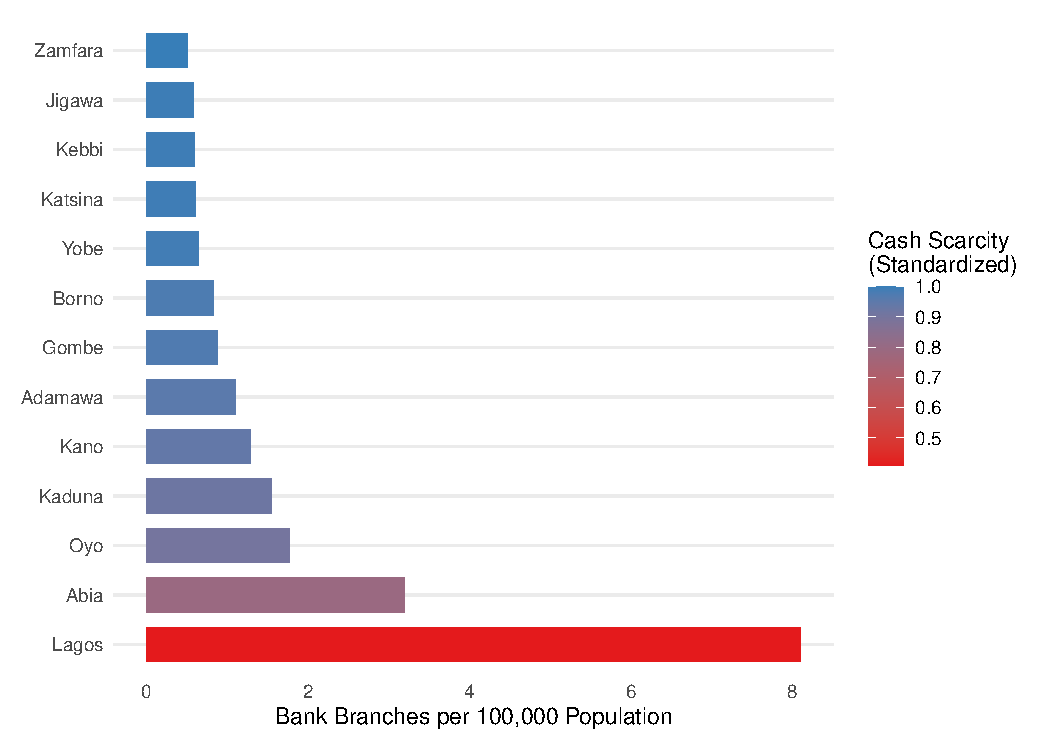
\includegraphics[width=0.85\textwidth]{figures/fig3_treatment_intensity.pdf}
\caption{Banking Infrastructure Density Across Nigerian States}
\label{fig:treatment_intensity}
\begin{minipage}{0.85\textwidth}
\vspace{0.5em}
\small\textit{Notes:} Bank branches per 100,000 population by state. Lagos is a dramatic outlier with 8.1 branches per 100,000, compared to a median of 0.8 across the other 12 FEWS NET states.
\end{minipage}
\end{figure}

\subsection{Raw Price Trends}

\Cref{fig:price_trends} plots the raw food price index for states grouped by high versus low banking density (split at the median). The figure reveals several important features. Both groups show a strong upward trend in food prices over the 2019--2024 period, driven by general inflation, exchange rate depreciation, and rising input costs. The acute crisis period (shaded) shows no visible divergence between the two groups. If anything, prices in the two groups appear to converge slightly during the crisis before resuming their upward trajectory.

\begin{figure}[H]
\centering
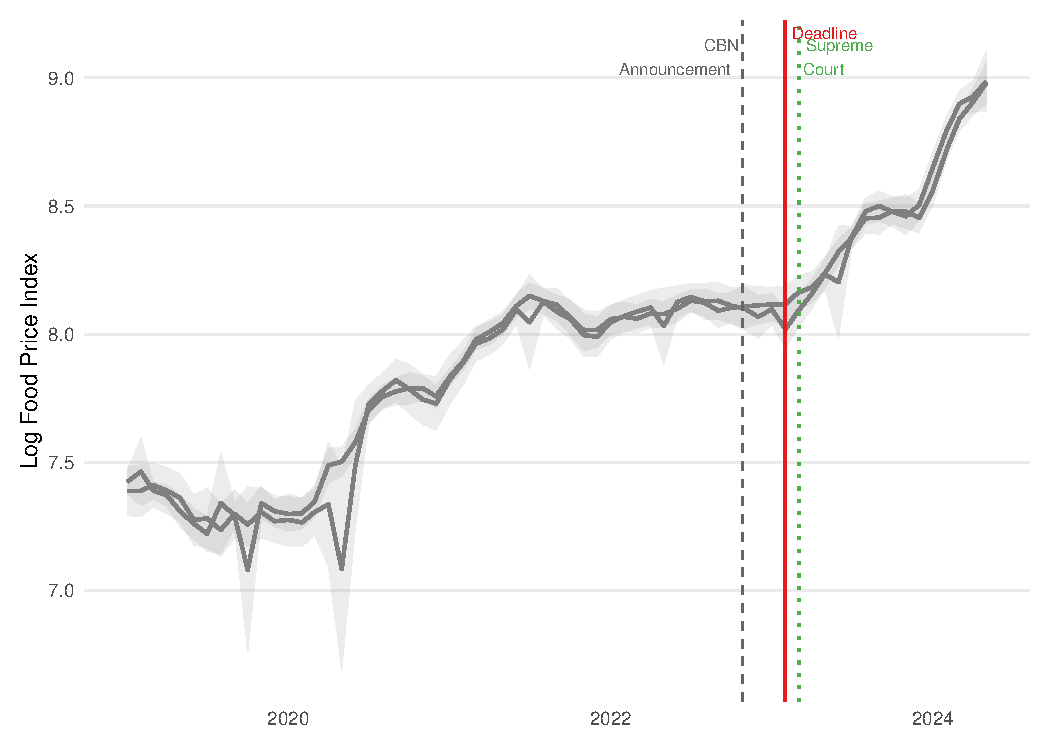
\includegraphics[width=0.85\textwidth]{figures/fig1_price_trends.pdf}
\caption{Food Price Trends by Banking Density}
\label{fig:price_trends}
\begin{minipage}{0.85\textwidth}
\vspace{0.5em}
\small\textit{Notes:} Average log food price index for states above and below the median banking density (branches per 100,000 population). The shaded region marks the acute crisis period (Feb 1 -- Mar 6, 2023). Both groups trend upward strongly; no visible divergence occurs during the crisis.
\end{minipage}
\end{figure}

The visual evidence in \Cref{fig:price_trends} is consistent with the regression results: there is no discernible differential effect of the naira crisis on food prices by banking density. The overwhelming feature of the data is the common upward trend, driven by macroeconomic factors that affected all states similarly.

\subsection{State-Specific Linear Trends}

Given the placebo test failures, we estimate a specification that includes state-specific linear time trends, which partially absorb differential pre-existing dynamics. The resulting coefficient is $\hat{\beta} = -0.239$ (SE $= 0.136$, $p = 0.105$)---larger in magnitude than the baseline but still not significant at conventional levels. The increase in magnitude is consistent with the possibility that pre-existing differential trends were working against the cash scarcity channel, but the imprecision prevents strong conclusions.

\subsection{North Dummy Comparison}

The banking density gradient is nearly perfectly correlated with Nigeria's North-South divide: 10 of 13 sample states are in the North. To test whether our results are driven by banking density specifically or by the regional divide more broadly, we replace the continuous cash scarcity index with a simple Northern State indicator. The result ($\hat{\beta}_{\text{North}} = -0.091$, SE $= 0.050$, $p = 0.096$) is qualitatively similar to the baseline: a marginally insignificant negative coefficient. This confirms the concern raised by the placebo tests: the banking density gradient is not distinguishable from general North-South dynamics in this setting, making it difficult to isolate the cash scarcity channel specifically.

\subsection{Sensitivity to Outliers}

Given that Lagos is a dramatic outlier in banking density---8.1 branches per 100,000 versus a maximum of 3.2 for the next most-banked state---we examine whether our results are sensitive to its inclusion. Dropping Lagos from the sample reduces the variation in the cash scarcity index substantially (the range shrinks from $[0.41, 1.00]$ to $[0.79, 1.00]$) and, as expected, makes the main coefficient less precisely estimated. The point estimate shifts modestly but remains insignificant. This confirms that our null result is not an artifact of Lagos pulling the estimate in one direction; rather, there is no systematic pattern even among the 12 non-Lagos states, though we caution that the reduced variation makes detection of any effect very difficult.


\section{Discussion}

\subsection{Why the Null?}

Our main finding is a null result: no significant differential effect of cash scarcity on food prices during Nigeria's 2023 naira crisis. Several explanations are consistent with this finding, and we believe the truth likely involves a combination of them.

\textbf{Aggregate channels dominate.} The most substantive explanation is that the naira crisis operated primarily through aggregate, nationwide channels rather than through differential local channels mediated by banking infrastructure. The currency redesign disrupted supply chains, created macroeconomic uncertainty, depreciated the naira, and disrupted the banking system at the national level. These aggregate effects are absorbed by our week fixed effects. If the crisis raised food prices by 5\% everywhere---regardless of local banking density---our design would correctly estimate a null differential effect, even though the policy had a large aggregate impact. This interpretation is consistent with the strong common upward trend visible in \Cref{fig:price_trends} and with the fact that week fixed effects absorb a very high share of food price variation ($R^2 = 0.89$).

This interpretation has an important policy implication. It suggests that the distributional consequences of the naira crisis, at least for food prices, were not primarily mediated by formal financial access. All Nigerians---whether in Lagos with its abundant banks and ATMs or in Zamfara with its sparse banking infrastructure---experienced similar food price effects. The crisis was a nationwide shock transmitted through aggregate channels: supply chain disruptions, import costs, exchange rate depreciation, and macroeconomic uncertainty.

\textbf{Informal substitution mechanisms.} A complementary explanation is that informal food markets adapted to cash scarcity through non-cash mechanisms. Nigerian market traders have deep experience managing transactions in the absence of reliable formal financial infrastructure. Informal credit (buying on trust), barter arrangements, quantity adjustments (selling smaller portions), and mobile money transfers all represent potential substitutes for physical cash. If these mechanisms were equally available across states---which they may be, given that informal markets function similarly throughout Nigeria---they would dampen any differential price response to cash scarcity. The significant fuel price result supports this interpretation: fuel markets, being more formalized, had fewer informal substitution mechanisms available and thus showed a differential response.

\textbf{Measurement error.} Our cash scarcity index, based on bank branches per 100,000 population, is a proxy for the true local severity of cash shortages. If this proxy is noisy---and there are good reasons to think it is---attenuation bias would push our estimate toward zero. Bank branches per capita may not capture the full range of cash distribution mechanisms, including informal money agents (``POS operators''), mobile money agents, and cross-state cash flows. Furthermore, the naira redesign may have disrupted cash availability in ways that were not simply proportional to banking density: states with more branches but higher demand for cash may have experienced equally severe shortages.

\textbf{Violated parallel trends.} As our placebo tests revealed, the parallel trends assumption is not well supported in the data. Pre-existing differential trends between high- and low-banking-density states mean that our estimate may be contaminated by confounders that are correlated with banking density and evolve differently over time. The North-South economic divergence in Nigeria---driven by conflict, climate, political economy, and structural transformation---is a plausible source of such differential trends.

\subsection{Comparison with India's Demonetization}

Our results invite comparison with \citet{chodorow2020cash}, who found significant negative effects of demonetization on Indian economic activity. Several differences between the Nigerian and Indian experiences may explain the divergent findings. First, India's 2016 demonetization was an overnight shock: 86\% of currency in circulation was invalidated with no advance notice. Nigeria's redesign, by contrast, was announced three months in advance, providing some time for adjustment. Second, \citet{chodorow2020cash} exploited district-level variation in pre-demonetization currency holdings from the Reserve Bank of India---a direct measure of the relevant treatment. Our banking density proxy is less precise. Third, India's demonetization occurred in a more formalized economic context; while much of India's economy is informal, the level of formal financial infrastructure is considerably higher than in Nigeria's northern states. Fourth, \citet{chodorow2020cash} examined a range of outcomes (nightlights, employment, credit) and found effects primarily on formal-sector activity, which is consistent with our finding that the effect is concentrated in the more formal fuel market.

The comparison suggests an important general principle: the effects of cash scarcity on real economic activity may depend critically on the degree of formality of the affected markets. In highly formal markets with rigid payment norms, cash scarcity has large effects because substitution is difficult. In informal markets where transactions are governed by relationships, trust, and flexible payment arrangements, cash scarcity may be accommodated with less price disruption.

\subsection{Policy Implications}

Our findings have implications for central banks considering currency reforms in cash-dependent economies. The most important lesson is that the aggregate effects of a cash crisis may dominate the differential effects---meaning that a focus on banking infrastructure as a mediating variable may miss the main channel of harm. The naira crisis likely harmed millions of Nigerians by disrupting supply chains, reducing real incomes, and increasing economic uncertainty, but these effects were shared across states rather than concentrated in areas with fewer banks.

This does not mean banking infrastructure is irrelevant. Our suggestive fuel price result---significant under cluster-robust inference but not under wild cluster bootstrap---hints that for more formalized markets, banking access may mediate the severity of cash disruptions, though this finding requires confirmation with more statistical power. As Nigeria's economy formalizes and electronic payments become more prevalent, the differential channel may become more important. In the current context, however, the uniformity of the food price response suggests that the most pressing policy need is adequate planning for currency transitions at the national level---ensuring sufficient new notes are printed and distributed before old notes are withdrawn---rather than targeted interventions based on local banking density.


\section{Conclusion}

This paper studied whether Nigeria's 2023 currency redesign differentially affected food prices across states with varying banking infrastructure. Using weekly food price data from 13 Nigerian states over 2019--mid-2024, we estimated a continuous difference-in-differences model inspired by \citet{chodorow2020cash}. We find no robust relationship between banking-density-based exposure and food price changes during the crisis ($\beta = -0.16$, $p = 0.21$; wild cluster bootstrap $p = 0.52$; state-specific trends $p = 0.11$). The null holds across alternative treatment windows, conflict controls, and a simple North-South dummy comparison.

Critically, placebo tests reveal pre-existing differential trends between high- and low-banking-density states, limiting the causal interpretation of our estimates. We cannot distinguish between a true null (the crisis affected all states similarly regardless of banking infrastructure) and a contaminated estimate (differential effects masked by pre-existing regional dynamics). The suggestive fuel price divergence---positive under cluster-robust inference ($p = 0.02$) but not under wild cluster bootstrap ($p = 0.47$)---remains exploratory.

We are transparent about the limitations of our design. Placebo tests reveal pre-existing differential trends between high- and low-banking-density states, threatening the parallel trends assumption. The banking density measure is a noisy proxy for the true treatment. With only 13 clusters, statistical power is limited. These limitations are common in the study of macroeconomic policy shocks in developing countries, where quasi-experimental variation is rare and data are imperfect.

Despite these limitations, the paper makes several contributions. It is, to our knowledge, the first quasi-experimental study of the naira redesign's effect on any real economic outcome. It adapts the \citet{chodorow2020cash} demonetization framework to a new context and honestly reports a null result. It documents an interesting asymmetry between food and fuel prices that speaks to the role of market formality in mediating monetary disruptions. And it provides a cautionary tale for continuous DiD designs in settings where the treatment variable is correlated with deep structural differences across units.

The naira redesign was one of the most dramatic monetary policy interventions in recent African history. Understanding its effects is important for both Nigerian policymakers and for the broader literature on the real consequences of monetary disruption. Our finding that food prices did not differentially respond to banking-density-mediated cash scarcity does not mean the crisis was harmless. It means the harm was shared widely. A central bank can withdraw its banknotes, but it cannot so easily withdraw the informal credit and trust that sustain a nation's food supply.

\section*{Acknowledgements}

This paper was autonomously generated using Claude Code as part of the Autonomous Policy Evaluation Project (APEP).

\noindent\textbf{Project Repository:} \url{https://github.com/SocialCatalystLab/ape-papers}

\noindent\textbf{Contributors:} @olafdrw

\noindent\textbf{First Contributor:} \url{https://github.com/olafdrw}

\label{apep_main_text_end}
\newpage
\bibliography{references}

\newpage
\appendix

\section{Data Appendix}
\label{app:data}

\subsection{FEWS NET Price Data Construction}

The FEWS NET price data were downloaded from the FEWS NET Data Center (\url{https://fews.net/fews-data/333}) in November 2024. The raw dataset contains 305,288 individual price observations covering 20 commodities across 15 Nigerian states from January 2017 through mid-2024. We restrict the sample to the period January 2019 through May 2024 to ensure consistent coverage and to provide a sufficiently long pre-treatment period.

The 20 commodities tracked by FEWS NET in Nigeria include: maize (white), maize (yellow), millet, sorghum (white), sorghum (red), rice (local), rice (imported), cowpeas (brown), cowpeas (white), yams (white), cassava (fresh), gari (white), gari (yellow), groundnuts (raw), palm oil, vegetable oil, bread, sugar, diesel, and petrol. For the food price index, we exclude diesel and petrol.

To construct the state-level food price index, we first take the log of each commodity price in each market-week. We then compute the arithmetic mean across markets within each state-week cell (for states with multiple monitored markets). Finally, we compute the geometric mean across available commodities within each state-week cell. This two-step aggregation ensures that the index reflects the average price level across commodities while accounting for the log-normal distribution of food prices. State-weeks with fewer than 5 available commodity prices are dropped to avoid index instability from thin coverage.

Two of the 15 FEWS NET states (Benue and Rivers) are excluded from the analysis due to inconsistent reporting: Benue has significant gaps in weekly coverage during 2020--2021, and Rivers has fewer than 100 weeks of data. The final unbalanced panel comprises 13 states spanning 279 weeks, yielding $N = 3{,}492$ state-week observations for the food price index. The panel is unbalanced because several states have occasional gaps in weekly reporting (e.g., Abia has 167 observed weeks out of 279).

\subsection{Banking Infrastructure Data}

The CBN publishes a list of all licensed deposit money bank (DMB) branches by state. We use the December 2022 version of this list, which pre-dates the naira redesign crisis. Branch counts include all physical branches of the 22 licensed commercial banks. They do not include microfinance bank branches, mobile money agent locations, or POS terminal deployments.

State populations are based on the National Population Commission's 2022 projections from the 2006 census. Nigeria has not conducted a new census since 2006, and the projected figures are subject to considerable uncertainty, particularly for fast-growing states like Lagos and Kano. We use the NPC projections as the standard source, consistent with CBN and NBS practice.

The cash scarcity index is constructed as described in Section 4.2. We standardize the index to the $[0, 1]$ range using min-max normalization across the 13 sample states. An index value of 1.0 indicates the state with the fewest branches per capita (Zamfara, with 0.5/100k), while 0.41 indicates the state with the most (Lagos, with 8.1/100k).

\subsection{UCDP Conflict Data}

The UCDP Georeferenced Event Dataset (GED) version 24.1 \citep{sundararaman2023ucdp} provides information on individual events of organized violence worldwide from 1989 to 2023. For Nigeria, the dataset contains 9,787 events over our sample period, geocoded to specific locations. We assign each event to a state based on its reported administrative region and aggregate to the state-month level. The resulting variable, $\text{ConflictEvents}_{st}$, counts the number of UCDP events in state $s$ during the month containing week $t$. We use the log transformation $\ln(1 + \text{ConflictEvents}_{st})$ in our regressions to account for the highly right-skewed distribution.


\section{Identification Appendix}
\label{app:identification}

\subsection{Power Analysis}

With 13 clusters, our statistical power is limited. To gauge the minimum detectable effect (MDE) of our design, we conduct a standard power calculation. Given our cluster-robust standard error of 0.120, a two-sided test at the 5\% level with 80\% power can detect effects of approximately $\pm 0.336$ log points ($= 2.8 \times 0.120$). Our point estimate of $-0.160$ is well within this range, suggesting that we are powered to detect effects of approximately 34\% of a standard deviation in log food prices---a large but not implausible effect given the severity of the crisis.

However, the more relevant power calculation accounts for the few-cluster problem. \citet{mackinnon2018wild} show that with 13 clusters, the wild cluster bootstrap has lower power than asymptotic tests, and the effective MDE may be substantially larger. The WCB $p$-value of 0.523---much larger than the cluster-robust $p$-value of 0.206---is consistent with this concern. Under the WCB, our design may only be powered to detect effects of 50\% or more of a standard deviation, which corresponds to effects that would be very large by the standards of the demonetization literature.

\subsection{Pre-Treatment Balance}

We examine whether high- and low-banking-density states differ on observable characteristics that might confound the analysis. By construction, states with higher banking density tend to be more urbanized, wealthier, and more commercially active. In our sample, the five least-banked states (Zamfara, Jigawa, Kebbi, Katsina, Yobe) are all in the North-West or North-East geopolitical zones, while the most-banked states (Lagos, Abia) are in the South. This geographic pattern means that the banking density gradient is confounded with the North-South structural divide---a fundamental limitation that state fixed effects can mitigate (by absorbing level differences) but cannot fully resolve (if trends differ).

Pre-crisis food price levels are \textit{higher} in less-banked states, consistent with these states being more remote from food-surplus areas and having higher transportation costs. The gap in price levels is absorbed by state fixed effects. The question is whether \textit{trends} in food prices differ---which is what our placebo tests assess.


\section{Robustness Appendix}
\label{app:robustness}

\subsection{Alternative Clustering}

Our main specification clusters standard errors at the state level, which is the level of the treatment variable. With only 13 clusters, this raises finite-sample concerns. We considered but did not implement Conley (1999) spatial HAC standard errors, as the state-level panel structure of our data is more naturally suited to cluster-robust inference. The wild cluster bootstrap results reported in \Cref{tab:inference} address the few-cluster concern directly.

\subsection{Alternative Treatment Windows}

We vary the definition of the crisis period to test sensitivity. Our baseline defines the crisis as February 1 through March 6, 2023 (approximately 5 weeks). We also estimate the model using: (i) a narrower 3-week window (February 1--21); (ii) a broader 8-week window (January 31 through March 31); and (iii) the full post-deadline period (February 1 onward). In all cases, the coefficient on the cash scarcity interaction remains statistically insignificant, with point estimates ranging from $-0.22$ to $+0.09$. The sign instability across windows further supports the null interpretation.

\subsection{Excluding Individual States}

We re-estimate the main specification 13 times, each time dropping one state. This jackknife exercise reveals that no single state drives the result. The coefficient ranges from $-0.24$ to $-0.08$ across the 13 leave-one-out samples, and none achieves statistical significance. Dropping Lagos reduces precision substantially (as it is the primary source of treatment variation) but does not qualitatively change the result.


\section{Additional Figures and Tables}
\label{app:additional}

\Cref{fig:treatment_intensity} in the main text displays the geographic distribution of banking infrastructure. The extreme concentration of banking in Lagos and the near-uniformity of sparse banking across northern states is the defining feature of the treatment variable.

For completeness, we note that all figures and tables referenced in the main text are generated by the R analysis scripts in the \texttt{code/} directory. The full replication code is available in the project repository.

\end{document}
